\begin{figure}[ht!]
\centering
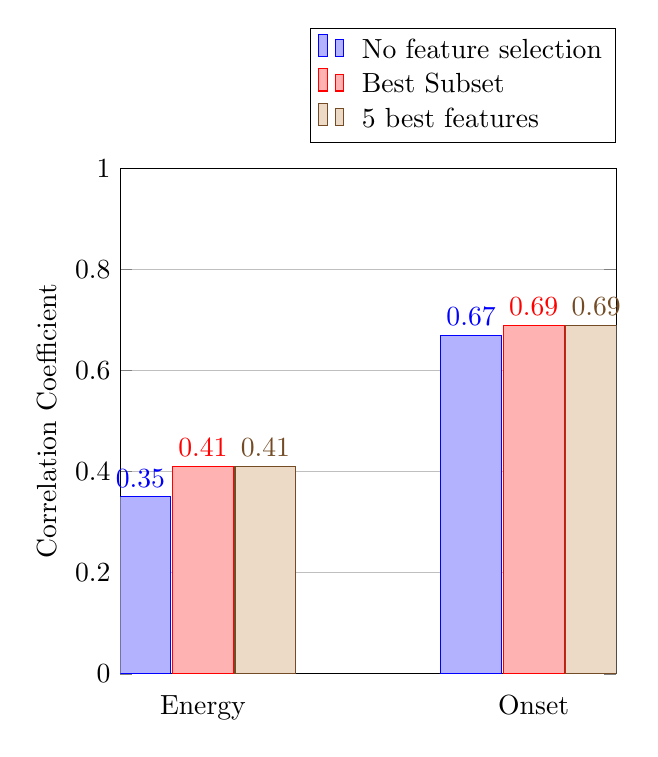
\begin{tikzpicture}
    \begin{axis}[
    	nodes near coords,
        width  = 0.65*\textwidth,
        height = 8cm,
        major x tick style = transparent,
        ybar=0.6,
        bar width=22pt,
        ymajorgrids = true,
        enlarge x limits = 0.5,
        ylabel = {Correlation Coefficient},
        symbolic x coords={Energy, Onset},
        xtick = data,
        scaled y ticks = false,
        enlarge x limits=0.25,
        ymin=0, ymax=1,
        legend cell align=left,
        legend style={
                at={(1,1.05)},
                anchor=south east,
                column sep=1ex
        }
    ]
        \addplot
            coordinates {(Energy, 0.35) (Onset,0.67)};

        \addplot
            coordinates {(Energy, 0.41) (Onset,0.69)};

        \addplot
            coordinates {(Energy, 0.41) (Onset,0.69)};


        \legend{No feature selection,Best Subset, 5 best features}
    \end{axis}
\end{tikzpicture}
\caption[Results with feature selection comparison.]{Results with feature selection comparison using Decision Trees. In this plot we use the "All" dataset.}
\label{fig:comparison}
\end{figure}